\documentclass{article}
\usepackage[utf8]{inputenc}
\usepackage{csquotes}
\usepackage[danish]{babel}
\usepackage{graphicx}
\usepackage{float}
\usepackage{pdfpages}
\usepackage{subcaption}

\usepackage{url}
 \usepackage{multicol}
\usepackage{hyperref}
\usepackage{cleveref}
\usepackage{natbib}

\usepackage{comment}

\usepackage{subcaption}
\usepackage{verbatim}
\usepackage{textcomp}




\title{Logbog \\ Social \& Æstetisk Interaktion}
\author{Karl-Emil Bilstrup, 201405858\\
Nicklas Nielsen, 201370312\\
Magnus Høholt, 201408770}
\date{\today}

% TIL 3D: Skriv mere på intro. Skriv kort afsnit om teknologi. Revider konklusion. Læs det hele igennem og se om du er tilfreds. Husk billeder.


% Noter til eksperiementer:
% Nuancerne ind i mellem. Lukkede af for omverdenen.
% De mistede alle fornemmelsen for tid.
% Forskellen mellem det abstrakte og konkrete 
% The uncanny valley?
% 3D verdenen blev men kameraet tiltede - især i tredje eksperiment
% Lyset i loftet - hvorfor så de det ikke?
% Kinect tracking blev mere og mere off
% Kinect skulle tracke kroppen først (T-form)
% Man kunne stjæle kroppe i forsøg 2 med Kinecten
% Sværere at tracke (ifht. kinect) når man sidder ned.
%   --> vi rykkede kinecten for at få bedre tracking
%   --> evt. flere kinects
% Heine kiggede ned af fordi HMD'en mistede tracking.
%   --> Der kan kun være 2 lighthouses
% Var det underligt at vi stod flere der inde?
%   --> Kun Jesper der spurgte.
%   --> De andre kommenterede ikke på det.
% VIVE'en er tung og det var forstyrrende.
% Spørgsmål er fra Vitmer - den Jonas snakkede om.
%   --> Brugt første skema 


% dNæNæ Latex-Template
% 
% Opret ny .tex fil til dit afsnit
% Brug \input{'filnavn'} for at indsætte fil
% Start filen med \Section{'Overskrift'}
% (De ovenstående ting er ordnet til EkspSys Afl.1)
% Skriv LaTeX som du ellers ville have gjort, men inde i filen
%
% Hvert afsnit bør (ifølge Kasper) opbygges således:
% 
% 1: Introduktion til metoden
% 2: Brug af metoden
% 3: Findings ved metoden
% 4: Metodekritik
%
% Jeg foreslår at afsnit 2-4 får egen subsection,
% men introduktion (på 2 linjer) skrives før første subsection.
%
% Vi forsøger så vidt muligt at undgår at skrive "vi", "os" og % så videre 
%
% Let the magic begin

\begin{document}

\maketitle

\setcounter{tocdepth}{2}

%\tableofcontents

\section{Koncept \& Prototype}

Dataman, se figur \ref{fig:Dataman} er en databank man har på sin person når man ønsker at indsamle alt data omkring ens færden, fysiske aktivitet og omgivelser. Dataman indsamler GPS koordinater, puls, temperaturer, lys niveauer, og optager alt lyd. Man kan på sin Dataman slukke og tænde manuelt for optagelse af data ved en on/off switch som viser sig som en oplys rød LED for at man ikke optager, og en grøn LED for at man optager. 
Man kan igennem et specielt håndtryk, udveksle data med hinanden. 
Alt data bliver visualiseret og styret igennem et interface på ens mobile enhed, eller computer, i form af en graf og en liste af rå data. Man kan slette data fra sin historik som man vil, men dette fremgår så som et hul i sin data historik. 
Man kan også sælge sin data. Det opbygger en vis værdi, som fluktuerer baseret på ens omgivelser og hvad man laver. F.eks. er dataen mere værd i centrum i en by omgivet af andre mennesker. Dataen for en pågældende dag bliver solgt hvis man vælger dette, man kan dog også vælge at donere sine data til et velgørende formål. 


\subsection{Prototype}
Dataman prototypen\ref{fig:Dataman} består af en Sparkcore enhed der indsamler data fra en temperatursensor, en puls sensor der sidder på spidsen af en finger, en lyssensor der måler lysniveauet, en lyd sensor der måler det generelle lyd tryk i ens omgivelser, og GPS koordinaterne fra ens tilkoblet enhed. Disse data sendes igennem wifi op til en cloudløsning fra producenten af sparkcore med HTTP igennem en API. Disse data tilgåes igennem samme API og bruges Javascript frameworket ReactJS. React formidler dataen op til HTML elementer som man så kan se live på en graf i ens browser, se figur \ref{fig:ui}. Dataen ses også som en løbende tabel under grafen. Data her kan slettes som man lyster.

\begin{figure}
    \centering
    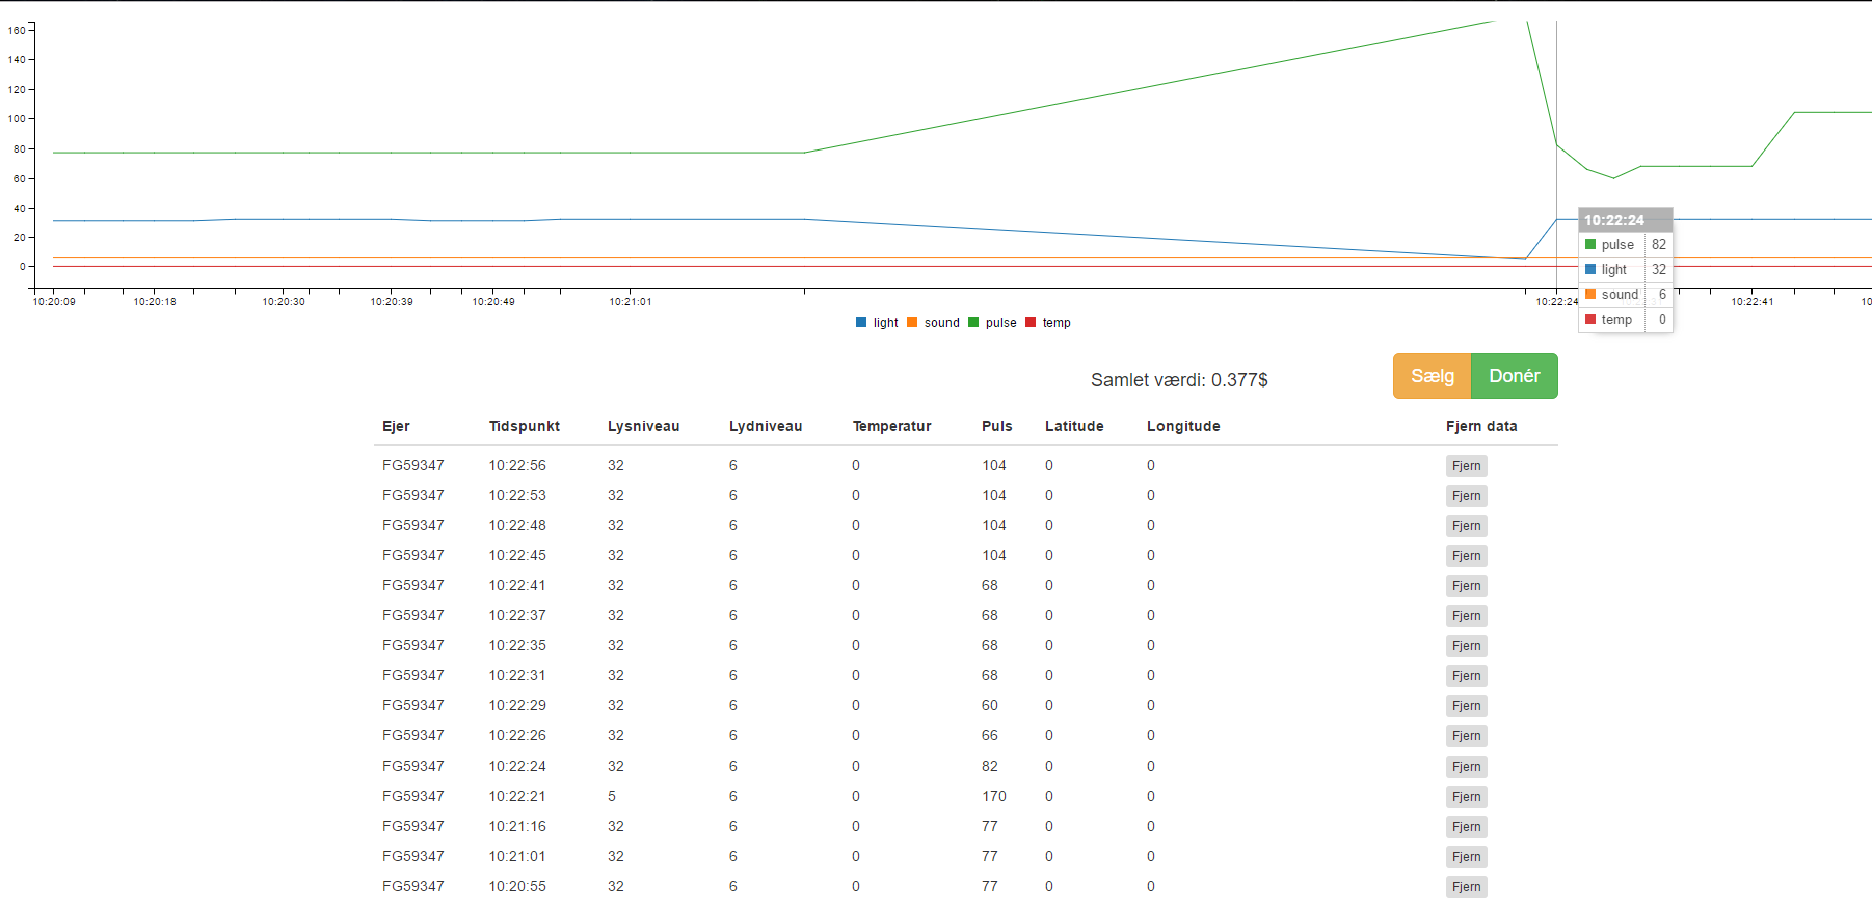
\includegraphics[width = \textwidth]{Pictures/datamanui.png}
    \caption{Datamans UI}
    \label{fig:ui}
\end{figure}

\begin{figure}
    \centering
    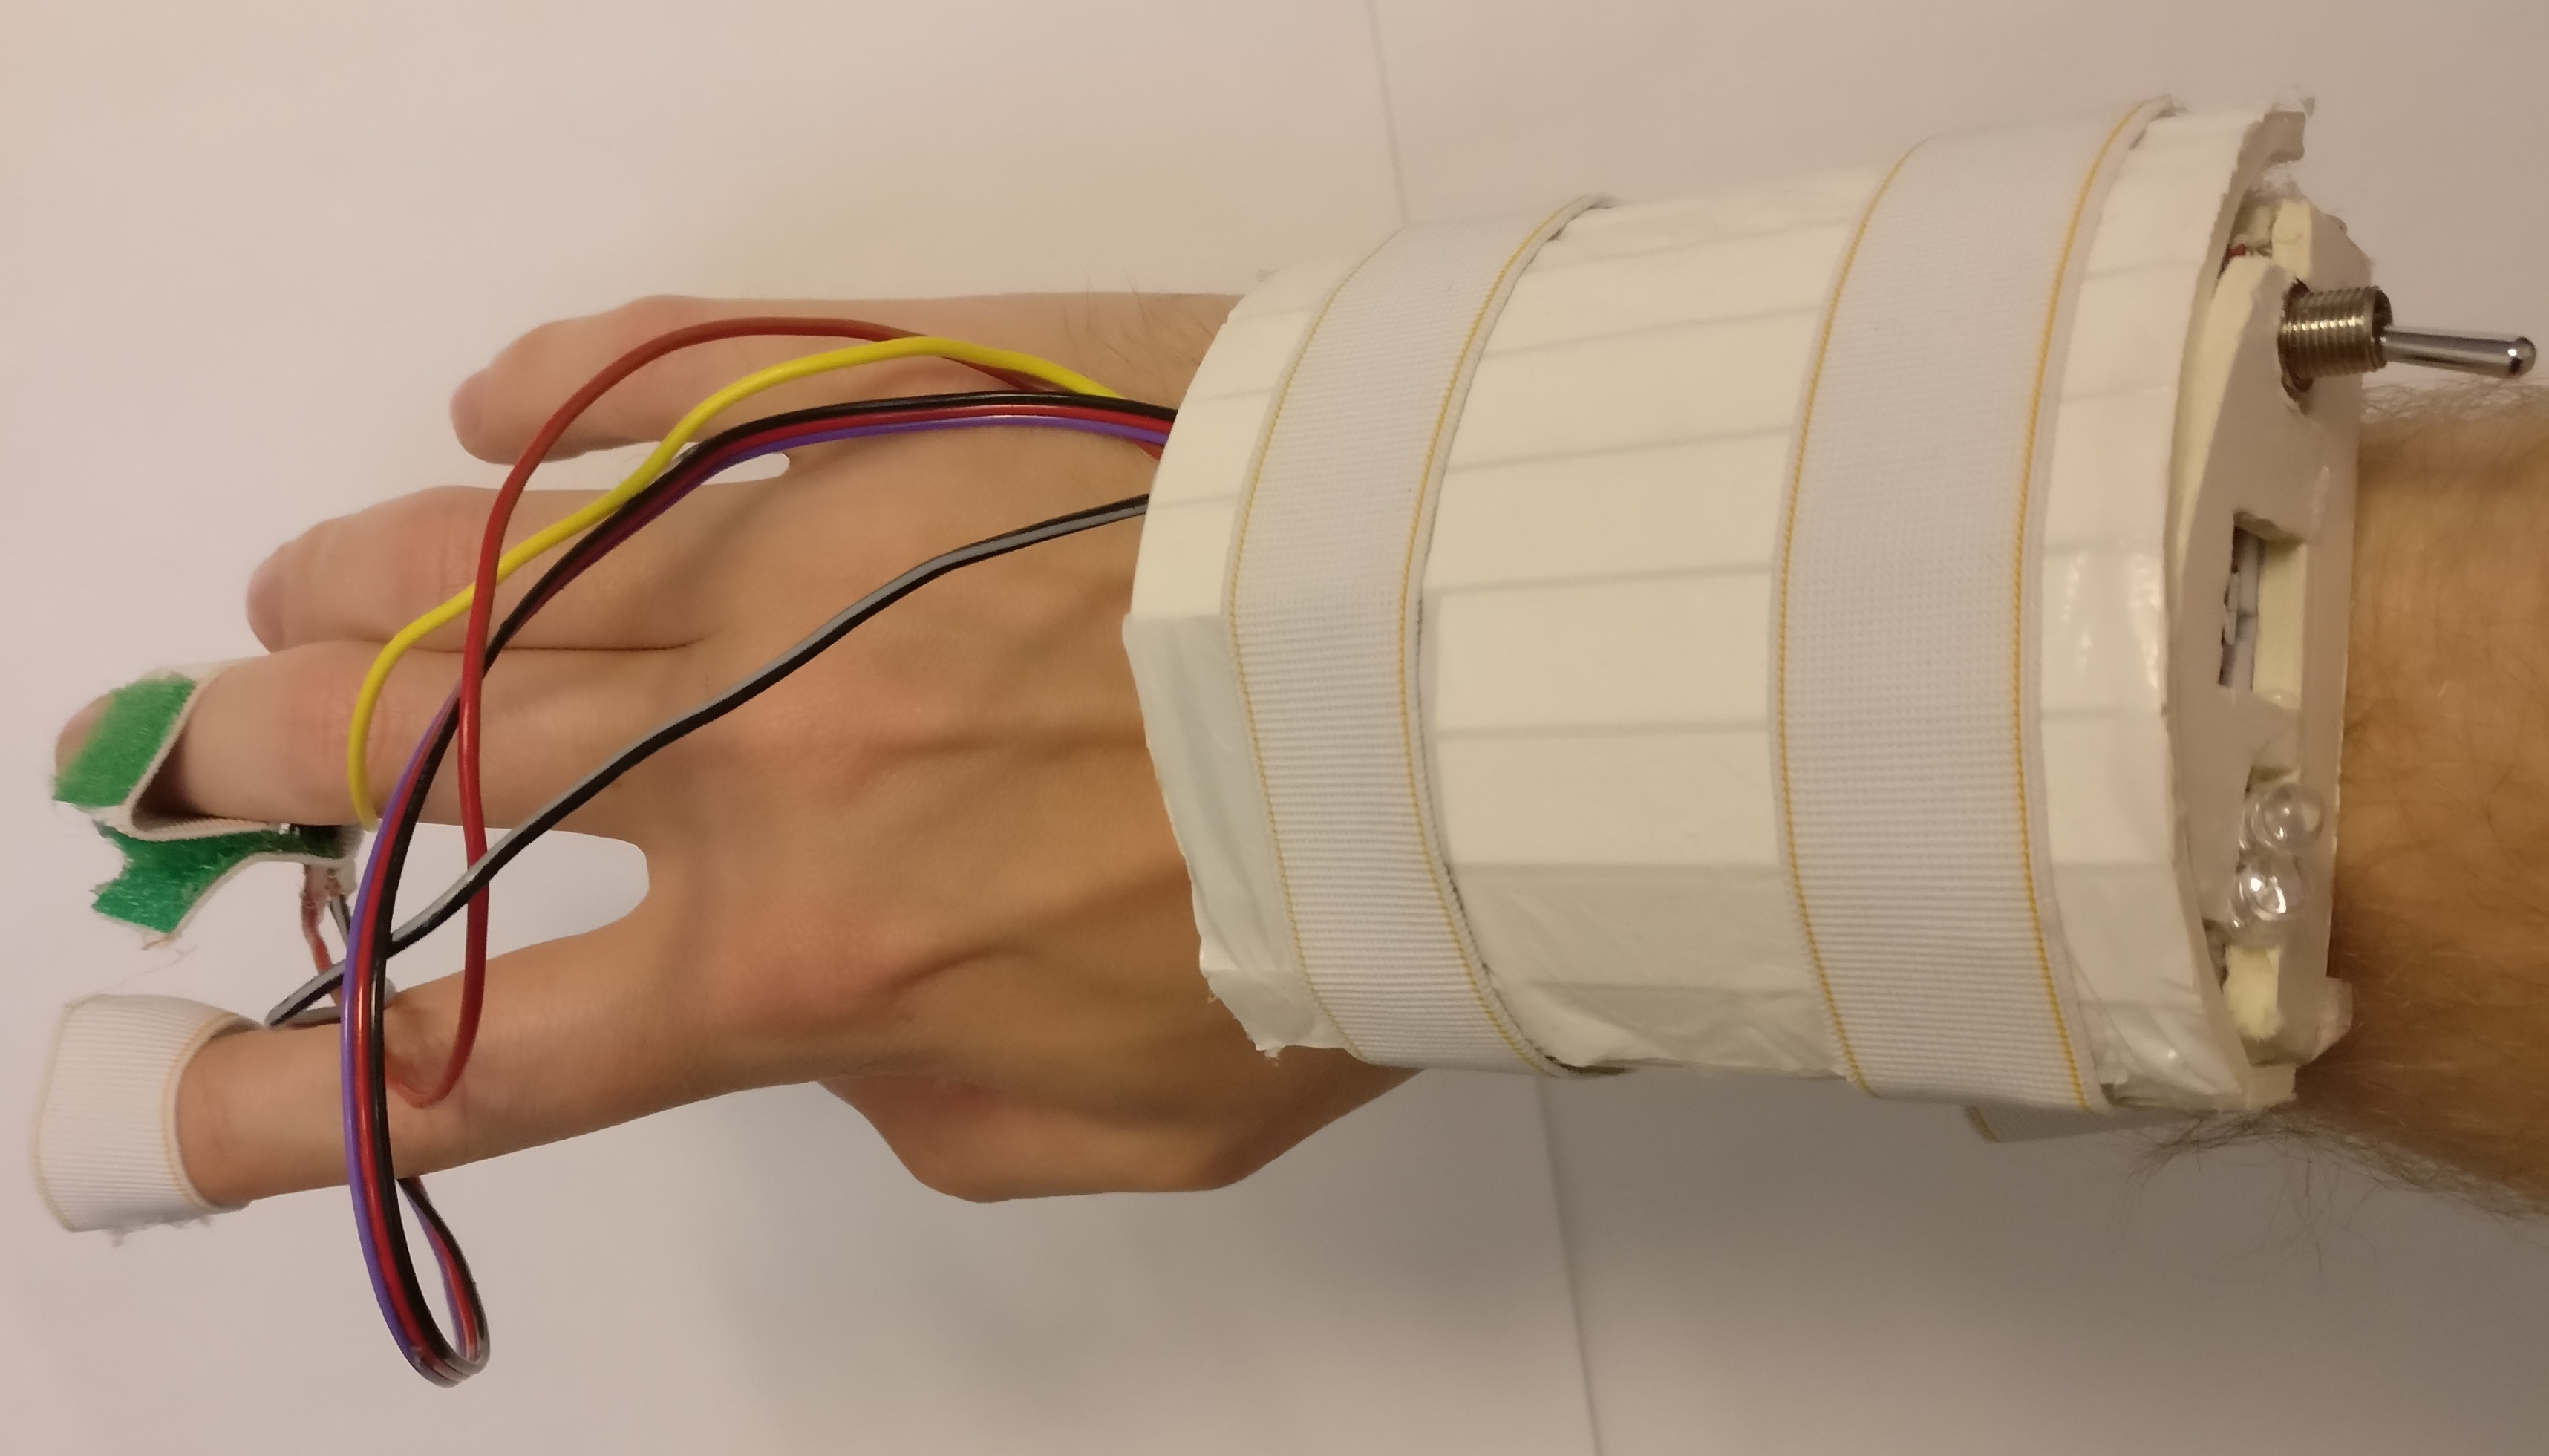
\includegraphics[width = \textwidth]{Pictures/Dataman.jpg}
    \caption{Dataman prototype}
    \label{fig:Dataman}
\end{figure}


\begin{comment}

HUSK AT SKRIVE OM WEBINTERFACE

\end{comment}

\section{Relevans}
Vi mener tryghed er en essentiel menneskelig følelse alle har ret til. Der er en direkte sammenhæng mellem tryghed og mentalt velvære. Når vi føler os utrygge er vi i beredskab, vi kan ikke slappe af, utrygheden tager vores fokus og kan potentielt overskygge alt andet. Kigger vi på Maslows behovspyramide~\cite[]{maslow}, ses det at tryghedsbehovet ligger tæt på nederst kun med fysiske behov under sig. Føler vi os ikke trygge falder behovet for det sociale, for vores ego og selvrealisering i baggrunden og vores energi bruges på at skabe tryghed, sikkerhed og stabilitet for os selv. For at et moderne samfund skal fungere og vi som mennesker, samfund og civilisation kan bevæge os fremad teknologisk og socialt, må vi føle os trygge. Trods dette må vi stadig overveje, hvordan vi skaber denne tryghed, hvilken form for tryghed vi er ved at skabe, hvem vi skaber tryghed for og på hvilken og hvis bekostning trygheden bliver skabt. 

%Social inno litteratur?

Der er i de seneste år flere eksempler på teknologier, der bruger Big Data til at overvåge det offentlige rum og bekæmpe kriminalitet og uorden for derigennem at skabe tryghed for samfundets borgere. Dette skaber nye problematikker og potentielle virkeligheder~\cite[]{Dunne:2013:SED:2613526}, vi som borgere i samfundet er nødt til at forholde os til. Nye teknologier gør det muligt at indsamle nye former for data. Fx indsamles der information fra sociale medier, der kigges på tidligere kriminelle begivenheder i geografiske områder og der optages lyd i bybilledet. Samtidig sættes flere og flere overvågningskameraer op. Dette skaber en enorm mængde data, som politiet eller andre kan tilgå. De kan dog umuligt analysere det manuelt. Derfor bliver data i højere grad analyseret af algoritmer, der hurtigt kan analysere og finde mønstre i de store datamængder. Dette har ført til en række produkter og løsninger, der er kommet på markedet de sidste par år. Fælles for disse løsninger er, at de symptombehandler uro og kriminelle tendenser. Big Data bliver brugt prædiktivt præventivt i opstående og eskalerende situationer og går generelt ikke dybere end dette. 

Eksempler på dette er CityPulse i Eindhoven~\cite[]{CityPulse} og SCAN NET i England~\cite[]{SCANNET}. CityPulse bruger realtidstracking af nattelivet med kameraer og mikrofoner samt realtidsanalyse af sociale medier som Facebook og Twitter til identificere optakt til uroligheder og stoppe dem i optakten. Fx ved at lyse området op. SCAN NET registrerer alle tilmeldte natklubbers besøgende med fingeraftryk og billede i en samlet database. Hvis en person får karantæne eller bliver smidt ud fra én natklub kan denne information tilgås af andre natklubber tilmeldt SCAN NET og dermed kan man udelukke individet fra samtlige natklubber baseret på en forseelse ét sted.

Et af de helt store buzzwords lige nu inden for bekæmpelse af kriminalitet er \textit{Predictive Policing}, hvor eksisterende data fra kriminalregistre, demografi, vejret og andet data bruges til at forudse, hvorhenne, i hvilket tidsrum og hvilken form for kriminalitet, der er mest sandsynlig. Et eksempel på sådan et system er PredPol~\textit{PredPol}, der anvendes i flere amerikanske storbyer til fortælle politiet, hvor de skal yde deres indsats og være synlige. I Danmark vil rigspolitiet begynde at tage Pol-Intel i brug i løbet af 2017. Pol-Intel er et Predictive Policing-system til at analysere kriminalregistre og sociale medier. Det er udviklet af Palantir, der også udvikler overvågningssytemer til bla. NSA, CIA og det amerikanske militær~\cite[]{PolIntel}. Politichef for rigspolitiet Svend Larsen argumenterer for, at politiet allerede i forvejen gør disse ting og at Pol-Intel blot effektiviserer det~\cite[]{Aflyttet}, men er det en valid argumentation, når effektiviseringen sker med en faktor 1000?


\begin{comment}

\end{comment}

\section*{Utopier}
Dorrestijn og Verbeek præsenterer et syn på, hvordan en higen efter det utopiske gennem design kan gøres relevant i vores samtid~\cite[]{dorrestijn2013technology} . Her præsenteres \textit{Nudging} og \textit{Persuasive Technology} som de to primære tilgange til adfærdsændring af folk gennem design. Dorrestijn og Verbeek foreslår en designmetodik, der fordrer \textit{opting-in} snarere end \textit{opting-out}, altså et tilvalg snarere end et fravalg. Denne måde at tænke på kan oversættes ganske nøjagtigt til problemstillingen om brugen af \textit{Big Data} til overvågning.

Nutidige ordensmagters tilgang til forhindring af kriminalitet er meget lig tilgangen i Nudging og Persuasive Technology. Brugen af vores data til det formål at beskytte os har skabt løsninger, der overser det enkelte menneskes behov og i stedet ser på os som dataindgange i et system, der så effektivt som muligt skal bekæmpe kriminalitet og skabe sikkerhed og tryghed. Dette systems syn på kriminelle er netop synet på kriminalitet som et tilvalg og altså synet på det retfærdige liv som fravalget af kriminalitet. Grundet dette syn bliver kriminalitet en handling, der skal forhindres og en kriminel, der jo selv har valgt kriminaliteten til, skal straffes eller i hvert fald rehabiliteres. Dette ses især tydeligt i PredPol-systemet, der netop hævder at kunne komme kriminalitet til livs ved at vide, hvor og hvornår den vil finde sted og derved forhindre den. På samme måde bliver tryghed en følelse som systemet udbyder. Denne følelse kan fravælges ved at stille sig uden for systemet (og blive kriminel), men den kan aldrig tilvælges. Som modpol, vil vi opstille et utopisk scenarie, der netop giver den enkelte borger mulighed for aktivt at deltage i et fællesskab, der i samarbejde opbygger en kultur omkring brugen af Big Data, og derved mulighed for at tilvælge sin egen retfærdighed og tryghed.

\section*{[a]- \& [b]-listerne}
For at nærmere at belyse den praktiske og politiske situation omkring brug af Big Data til at skabe tryghed, har vi fundet inspiration i Dunne \& Raby's [a]- \& [b]-lister \cite[]{ABList}. Først vil vi præsentere en [a]-liste, der eksemplificerer den praksis vores samfund ultimativt bevæger sig imod ved at  opsummere kendetegnene ved den tilgang, systemet i dag har til Big Data som værktøj til at skabe tryghed. Senere vil vi præsentere en [b]-liste, der opsummerer en modpol til [a]-listen og tegner en anderledes utopi for brugen af Big Data.

\subsection*{[a]-listen}
PredPol, CityPulse og snart Pol-Intel bygger alle på samme præmis. Ved at være tilstede, hvor og når kriminaliteten sker, kan man afværge forbrydelser og uro. Ved at afværge forbrydelser, vil kriminaliteten falde. Myndighederne skal altså kunne træde ind og \textit{beskytte} borgerne mod kriminelle handlinger, der vil give dem ubehagelige og utrygge oplevelser. %Følges denne tilgang til dør, bliver det myndighedernes opgave at beskytte befolkningen, der ultimativt aldrig vil opleve kriminaliteten, fordi myndighederne kan stoppe den, før den er sket. 
Ultimativt giver det myndighederne et monopol på tryghed, da borgeren aldrig får muligheden for at skabe deres egen tryghed. Alt indsamlet data ejes af systemet og bruges af den lovopretholdende indstands, der forudsiger kriminaliteten ved at analysere de store mængder data for at pege på hvem, hvornår, hvor og hvad. %Dette fører til en stigmatisering, hvor myndigheder bestemmer, hvem der er kriminelle, da de har eneret på denne data. 
Borgerne kan blot forsøge at holde sig i mængden af de lovlydige, så de ikke kommer i myndighedernes søgelys og potentielt bliver udpeget som kriminelle. Nedenfor har vi listet disse pointer i en [a]-liste.

\begin{figure}[H]
        \begin{itemize}
            \item[] \textbf{[a]}
            \item Tryghed oppefra
            \item Tryghed er tilliden til systemet
            \item Symptombehandling
            \item Skabe ro og orden
            \item Systemet beskytter individet
            \item Systemet afværger kriminalitet
            \item Systemet profilerer individer
            \item Data ejes af systemet
            \item Data bruges af systemet
            \item Kortsigtet~\textrightarrow~nu og her
        \end{itemize}

    \caption{[a]
    -listen}
    \label{fig:a_liste}
\end{figure}


For at få en dybere forståelse af denne praksis, kan vi bruge Meadows' Leverage Points~\cite[]{LeveragePoints}. Der ses en tendens til generelt at bruge Big Data til løsninger med et kort \textit{delay}. Nye værktøjer til at bekæmpe kriminalitet og skabe tryghed skal gerne skabe resultater hurtigst mulig for at bevise deres værd. PredPol reklamerer på deres hjemmeside med at mindske kriminalitet på få måneder~\cite[]{PredPol}. Dette gøres ved at ændre \textit{The Structure of Information Flows}, hvor information udledt fra Big Data transmitteres direkte til de personer, der skal opretteholde lov og orden.

Fjernes disse nye værktøjer, som PredPol eller CityPulse, fra systemet vil deres påvirkning på systemet øjeblikkeligt forsvinde. Kan ordensmagten ikke længere være til stede til at afværge de kriminelle handlinger, vil de opstå som før og utrygheden vil genopstå. Måske endda i endnu højere grad, da borgerne vil have mistet en del af deres ansvarsfølelse under ordensmagtens kontrol. 


\subsection*{[b]-listen}
I [b]-listen præsenterer vi en alternativ praksis, hvor vi gennem en \textit{reframing} af problemet~\cite[]{FrameInnovation} vil vise en anden tilgang til systemet: I stedet for at se tryghed som myndighedernes ansvar, skal tryghed tilhøre borgerne og fællesskabet. Inspireret af Dorrestijn \& Veerbeek~\cite[]{dorrestijn2013technology} vil dette blive et distribueret system, hvor ansvaret for trygheden ligger hos det enkelte individ og kun gennem fællesskab kan en samfundsrækkende tryghed skabes.

Dette kræver, at borgerne får de nødvendige værktøjer og information samt en fælles bevidsthed om et fælles ansvar. Denne indsigt opnås ved at flytte ejerskabet af den data, der genereres af moderne teknologi fra systemet til individet selv. Således flyttes også ansvaret for denne datas anvendelse til individet, og det er kun gennem aktiv deltagelse i et større fællesskab, at denne data bliver anvendelig\footnote{Dette kan i sagens natur ses som én stor tillidsøvelse borgere i mellem. Der er en overhængende risiko for at ekstreme bevægelser vil forsøge at få den endelige magt over samfundet. I bund og grund er dette et grundlæggende problem med socialistiske projekter og konsekvenser af dette har været gennemsyrende for vores globale samfund gennem det 20. århundrende.}.

Konsekvensen af dette system vil være en anvendelse af Big Data, hvor hvert enkelt individ vil blive hørt, fordi det i sagens natur er medejer af systemet. %I stedet for at behandle borgerne som rækker og kolonner i et system, bliver borgerne udgangs- og omdrejningspunktet for det fællesskab, der danner grundlaget for et trygt samfund. 
Bryder enkelte medlemmer af fællesskabet sammen, vil det resterende fællesskab løfte individet i flok, da det er afhængigt af det enkelte individ. Denne samfundsstruktur er manifesteret i [b]-listen nedenfor, hvor det ses sammenholdt med [a]-listen.

\begin{figure}[H]
    \centering
    
\begin{multicols}{2}
\begin{itemize}
    \sloppy
    \item[] \textbf{[a]}
    \item Tryghed oppefra
    \item Tryghed er tilliden til systemet
    \item Symptombehandling
    \item Skabe ro og orden
    \item Systemet beskytter individet
    \item Systemet afværger kriminalitet
    \item Systemet profilerer individer
    \item Data ejes af systemet
    \item Data bruges af systemet
    \item Kortsigtet~\textrightarrow~nu og her

    \item[] \textbf{[b]}    
    \item Tryghed nedefra
    \item Tryghed er tilliden mellem individer
    \item Skabe en fælles kultur
    \item Gro gensidig forståelse
    \item Fællesskabet oplyser individet
    \item Fællesskabet løser konflikter
    \item Individer hjælper hinanden
    \item Data ejes af individet
    \item Data bruges af fællesskabet
    \item Langsigtet~\textrightarrow~selvopretholdende
    
\end{itemize}
\end{multicols}
    \caption{[a]- \& [b]-listen}
    \label{fig:a_b_liste}
\end{figure}

\noindent Informationsflowet i denne nye virkelighed er altså radikalt anderledes end det tidligere. I stedet for at lade information flyde fra borgerne til de offentlige instanser, vil informationen flyde mellem borgenerne og skabe en bedre forståelse imellem dem. Effekten af overgangen til et sådant system vil have et langt \textit{delay} og ikke mindske kriminaliteten på få måneder. I stedet vil denne nye samfundsstruktur have en langsigtet og selvopretholdende effekt, hvor trygheden ikke vil være afhængig af enkelte faktorer, men indbygget i kulturen. På denne måde bliver målet at skabe et samfund og en kultur, hvor ingen vil begå kriminalitet.

\subsection*{En bedre forståelse}
%Vi har opstillet [a]- \& [b]-listen, der står som modsætninger til hinanden, hvor [b]-listen lige nu er en ren utopi, der ligger langt fra den virkelighed, vi lever i. Ikke rent teknologisk men kulturelt og menneskeligt. 
[a]- \& [b]-listen udspænder et spektrum fra det ene ekstrema til det andet. Som beskrevet tidligere har nye teknologier ført til, at vi har flyttet os mod en virkelighed, der minder mere om [a]-listen. Dette er sket og sker uden nogen offentlig debat om, hvorvidt det er den retning, vi ønskeligt vil bevæge os i. Teknologien kan sagtens bruges anderledes, men vi følger tilsyneladende nogle mønstre og tankesæt, der fører os i denne retning. Se illustrationen i figur[FIGUR].

\textit{Dataman} skal hjælpe brugeren til at bryde ud af disse ubevidste mønstre og tankesæt, til at se der er flere retninger vi kan bevæge os i og ultimativt til at tage aktivt stilling. Figur [FIGUR] illustrere dette i en repræsentation inspireret af Dunne \& Rabys diagram over mulige fremtider~\cite[]{Dunne:2013:SED:2613526}.

Det er styrkelse af det enkelte individ, hvor han selv kan vælge hvor meget data han genererer, hvilken data han vil generere, hvornår han vil generere data og hvad han vil bruge den til. Det er en lille lomme af kontrol i et samfund, hvor vi ellers sjældent har kontrol over vores data. Vi kan selv tilvælge overvågningen \cite[]{dorrestijn2013technology}. Det er en ekstrem overvågning af os selv, men vi er samtidig i total kontrol af denne overvågning. Vi behøver ikke at vente på omverdenen. Vi får mulighed for at tage aktive valg nu og her. Det er måske kun omkring vores egen lille lomme af data, men vi kan rent faktisk tage et valg og føre det ud i livet inde i denne lille lomme.

%HER HAR MAGNUS TILFØJET TING. LÆSES IGENNEM?
\section*{Socioæstetiske overvejelser}
Modsat andre prototyper (se afsnittet Designproces) er Dataman ikke afhængig af et fællesskab for at fungere, men optager altid data omkring brugeren. Dog kan brugeren drage nytte af fællesskabet. Når to brugere af Dataman mødes og giver hinanden hånden, udveksles en smule data mellem de to brugere og dermed bekræfter de hinandens data.

Håndtrykket har siden middelalderen været en gæstus af høj symbolsk værdi\footnote{\url{https://www.kristeligt-dagblad.dk/liv-sj\%C3\%A6l/vi-giver-h\%C3\%A5nd-til-ligem\%C3\%A6nd}}.

\begin{displayquote}[Inge Adriansen, PhD i Nordisk Folkemindevidenskab]
\textit{De sammenlagte hænder er et stærkt og letforståeligt symbol. Det er et tegn på gensidighed og et ligeværdigt forhold, da begge parter udfører den samme handling.}
\end{displayquote}

Også i dag er håndtrykket en vigtig del af det sociale liv. Håndtrykket er altafgørende for, hvilket førstehåndsindtryk, vi danner os om de mennesker, vi møder. 

Dataman udnytter denne symbolik og påfører den endnu et aspekt. Når du giver hånden til en anden person, eksponerer du en lille del af dig selv. Meget konkret får den anden person adgang til noget data omkring dig. Håndtrykket bliver derfor i endnu stærkere grad et symbol på tillid og gensidighed. Du ville vel ikke give en person, du ikke stoler på adgang til \textit{din} data? Og kan du egentlig stole på en person, der skjuler sin data fra dig? Dataman forsøger ikke at svare på disse spørgsmål, men giver i stedet brugeren mulighed for, at opdage og overveje disse problemstillinger selv.

Som beskrevet tidligere er indikerer Dataman sin optagen ved hjælp af en lysende diode. Grøn når der optages, rød når der ikke gør. På denne måde, kan omgivelserne nemt se, om brugerne af Dataman optager eller ej. Omgivelserne må så selv afgøre, hvordan de vil reagere på en sådan bruger. Ville du gå hen og snakke med en fremmed, du vidste optog jeres samtale? Ligeledes kan brugeren reagere på sine omgivelser. Hvis hun gerne vil kommunikere fortrolighed kan hun slukke optagelsen på sin Dataman. Modsat kan hun tænde den, hvis hun står i en utryg situation, hun gerne vil dokumentere.

Den data, Dataman genererer, kan tilgås gennem et web interface. Man har altså altid adgang til sin tidligere data. Denne data kan som beskrevet manipuleres, slettes, sælges eller doneres. Faktisk er der ingen grænser for, hvordan ens data kan bruges. Man ejer det jo selv. Hvad nu, hvis din kæreste spurgte, hvor du var henne i går? Hvad hvis hun ikke stolede på, hvad du sagde og forlangte at se data, der bekræftede det? Hvad hvis du have slettet den data? Ellers solgt den?

Dataman følger med, hvorend brugeren går. Derfor indgår den også i flere forskellige sociokulturelle kontekster og vil have forskellige betydninger i forskellige kontekster. Dette stemmer ens med \cite[]{Petersen:2004:AIP:1013115.1013153}, der netop argumenterer for, at den æstetiske oplevelse ved et designartefakt ikke kun kan ses i isolation, men skal forstås i en brugskontekst. Vi vil altså argumentere for, at Dataman i høj grad er æstetisk i en sociokulturel forståelse af begrebet.

%Der opstår nogle sociale overvejelser. ... æstetisk interaktion...

%Håndtrykket??

\section*{Forskellige typer tryghed}
Til at arbejde med forskellige typer af tryghed har vi opstillet et diagram, der viser, hvem der tager initiativet til at skabe tryghed, og hvordan denne tryghed skabes. Trygheden kan enten skabes gennem kontrol eller gennem tillid og initiativet kommer enten fra individet eller fra fællesskabet. Fællesskabet kan i nogle tilfælde være repræsenteret af andre. I [a]-listen er det fx systemet, der varetager fællesskabets interesser. Diagrammet kan ses i figur [FIGUR], hvor [a]- \& [b]-listen også er plottet ind. 
    


\begin{comment}
 

%Det sjove videokort

%Det handler om overvågning
%Smart cities generelt
%NOGET OM POL INTEL!
%opdater a og b listerne til det nyeste
%Social inoovation (Nicholls and mudic tekst)
%De to akser symboliser forskellige former for tryghed
\end{comment}
\section*{Designproces}
\label{section:designproces}
I det følgende afsnit, vil vi præsentere, hvordan vores designproces mod Dataman som koncept har udspillet sig. I vores designprogram (se bilag), har vi fremlagt den arbejdsproces vi forestillede os, baseret på \cite[]{bang2012role}'s procesmodel, som ses i figur \ref{fig:procesmodel}.

\begin{figure}
    \centering
    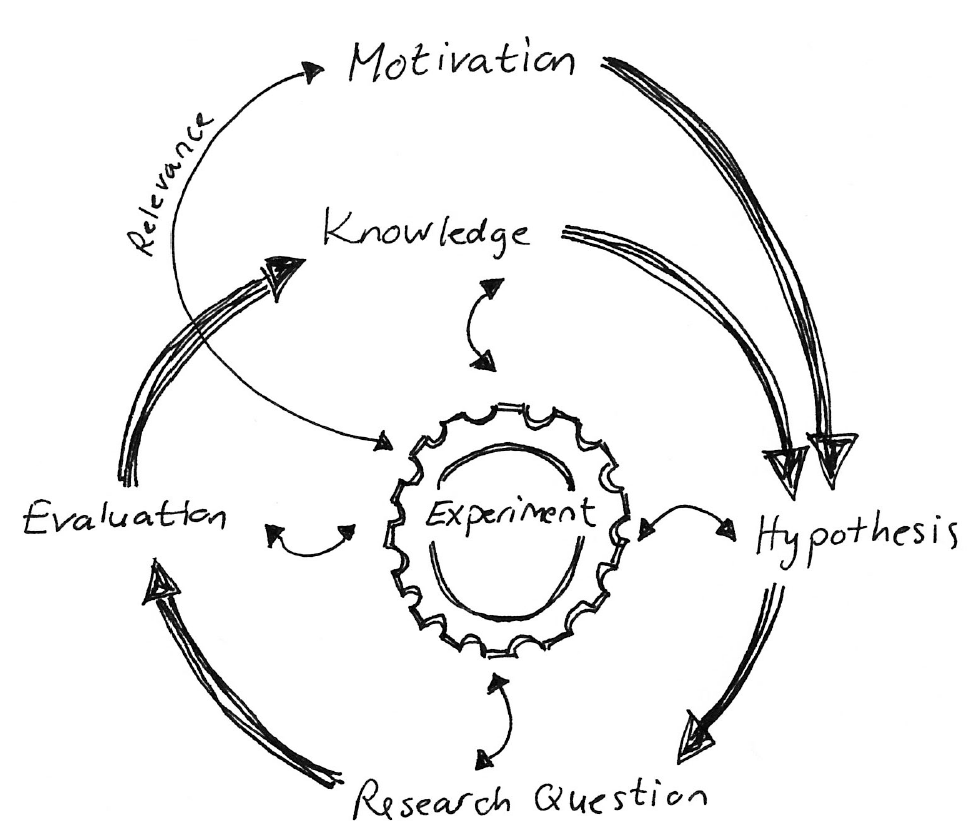
\includegraphics[width = \textwidth]{Pictures/PetersProcesModel.png}
    \caption{\cite[]{bang2012role}'s model over en designproces}
    \label{fig:procesmodel}
\end{figure}

Den rent faktiske proces har, som oftest tilfældet, vist sig at være mere rodet end først antaget. Af denne årsag, har vi brugt modellen fra figur \ref{fig:procesmodel} som analyse værktøj til processen. I dette afsnit vil denne proces blive fremlagt og hvert eksperiment vil blive analyseret med inspiration fra \cite[]{krogh2015ways} med henblik på, hvordan processen har ændret sig på baggrund af eksperimentet - hvordan vi har \textit{drift}et.

\subsection*{Forarbejdet}
Projektet udsprang fra et ønske om, at beskæftige os med tryghed og nattelivet. For at undersøge konteksten nærmere, bevægede vi os ud i nattelivet for at observere, hvordan og om folk følte sig trygge. Denne observation udførtes i tråd med \cite[]{suri2005thoughtless}'s tanker om intuitiv observation. På baggrund af observationerne undersøgte vi konteksten nærmere for statistikker og artikler. På trods af meget lav kriminalitet i Danmark\cite[]{LavKrim} oplever danskerne en højere utryghed \cite[]{HoejUtryghed}. Det fortæller os, at den  nuværende indsats overfor tryghed ikke virker optimalt, og at der er rum til nytænkning. Århus, hvori vi udførte observationen, er rangeret som den by (af de 5 største) der har relativt færrest trygge borgere i 2016\cite[]{KrimStat}.
Herefter undersøgte vi, hvilke tiltag, der i dag blev taget for at bekæmpe utryghed og kriminalitet i Danmark og i udlandet. Den mest udbredte metode er her det såkaldte prædiktive politiarbejde \cite[]{PredPol,CityPulse, PolIntel}.

Ud fra denne viden opstillede vi en hypotese om, at konsekvenserne af ukritisk brug af Big Data er mange og uoverskuelige, fordi Big Data per definition er uoverskueligt. På baggrund af denne hypotese udarbejdedes en række skitser, der undersøgte designrummet udspændt af temaerne; Big Data, Nattelivet og Tryghed (skitserne kan findes i vores designprogram i bilaget). I udformningen af disse skitser arbejdede vi ved hjælp af \textit{probing} (se \cite[]{krogh2015ways}), hvor vi frit og ustruktureret undersøgte designrummet muligheder. Dernæst foretog vi en kort intern evaluering af skitserne og arbejdede \textit{akummulativt} med at udfolde nogle af de koncepter skitserne indeholdt.

Dette eksperiment førte os til en ny erkendelse. Mange af vores skitser indebar en fremskrivelse af verdens nuværende brug af Big Data og disse skitser var dystre og tegnede et nærmest orwellsk syn på fremtiden. Ud fra dette, vores tidligere undersøgelser og med inspiration fra \cite[]{Dunne:2013:SED:2613526}'s [a] og [b]-liste over spekulativt design opstillede vi vores egen [a]- og [b]-liste, der repræsenterer to ekstreme fremskrivninger af brugen af Big Data. Her opstod en ny hypotese: Ved, som nu, ukritisk brug af Big Data bevæger vi os som samfund mod [a]-listen.

På baggrund af listerne stiller vi os selv spørgsmålet; hvad nu, hvis vi i stedet bevægede os mod [b]-listen? Hvordan ville et samfund så se ud? Og hvordan ville Big Data være realiseret i et sådant samfund? Vi arbejdede her kort videre med skitserne fra tidligere. Her arbejdede vi \textit{ekspansivt} med at udfylde de områder i designrummet skitserne ikke dækkede, for på denne måde at sandsynliggøre [b]-listens samfund.

\subsection*{Fremtidsværkstedet}
Dernæst udførte vi den første af to workshops med inspiration fra Participatory Design. For at se hvordan brugere af nattelivet oplever tryghed i kontekst af Big Data, udførte et fremtidsværksted~\cite[]{PD}, hvor vi fremlagde de tidligere nævnte projekter som inspiration til debat. Til inpiration præsenteredes [b]-listen samt skitser af enkelte koncepter og scenarier som mulig provokation af deltagerne. Deltagerne forholdt sig dog ganske ukritiske overfor nuværende projekter og brugen af deres data i kontekst af nattelivet. De var generelt positivt stemt overfor mere institutionel brug af Big Data for at skabe mere tryghed, da de forstod dette som en effektiv måde at skabe mere effektiv overvågning. Deltagerne accepterede altså ikke vores præmis om den nuværende situation, som en de burde være skeptiske omkring.

Denne erkendelse førte til et større skred i vores designarbejde. Hvor vi før havde arbejdet under hypotesen om, at hvis blot vi fremlagde samfundssituationen for den almindelige borger, ville de forstå, hvorfor denne kunne føre til et uønskeligt samfund. Dette var i lyset af vores fremtidsværksted dog ikke tilfældet. Derfor ændrede vi vores arbejdshypotese: Vi lever i dag i et overvågningsparadigme, hvor overvågning ses som det bedste og potentielt eneste måde, at komme utryghed til livs. Vi stillede derfor os selv spørgsmål: Hvordan får vi den enkelte borger til at tage kritisk stilling til konsekvenserne ved brugen af Big Data til overvågning?

Vi ville afsøge det nye spørgsmål ved at præsenter et produkt der lå over mod [b]-listen og lade dem stå som kontrast til den retning vi bevæger os imod i dag. Dette krævede dog en undersøgelse af, hvor på på spekteret mellem [a]- og [b]-listen dette produkt skulle ligge for blive accepteret som et reelt produkt, men stadig male kontrasten. For at undersøge denne tilgang ville vi \textit{serielt} bevæge os frem og tilbage på spekteret. Vi besluttede os for at starte så langt ude mod [b]-listen som vi kunne komme.

\subsection*{Den første iteration}
Med dette nye fokus opstillede vi to nye eksperimenter i form af to produkter, der skulle realisere [b]-listens samfundsmodel; CityMood og TOTEM. I brugen af begge produkter indgår brugeren i et fællesskab med andre brugere. CityMood[BILLEDE] er en app, der viser alle medlemmerne af dets fællesskab på et samlet kort. Formålet er at skabe et trygt byliv, og app'en kan derfor vise brugeren, hvilket humør de andre medlemmer er i, samt hvordan brugeren ville klinge sammen med enkelte medlemmer. TOTEM er et pandebånd, der ved hjælp af en unik sammensætning af sensorer, kan aflæse dine følelser. Disse følelser bliver udsendt og påvirker således andre medlemmer af fællesskabets følelser. Brugeren selv bliver altså ligeledes påvirket af resten af fællesskabets følelser.

Vi udførte en intern evaluering af de to koncepter og besluttedes os for at forsætte med TOTEM-konceptet, da det indholdt flest værdier fra [b]-listen. Ud fra TOTEM konceptet designede vi TOTEM v2, der brugte data generet af fællesskabet i nærheden af brugeren til at generere et abstrakt lydunivers, der kunne gengive stemningen omkring brugeren. På denne måde kunne brugeren få en oplevelse af, hvordan fællesskabet omkring hende havde det - og potentielt ændre adfærd og handle aktivt på baggrund af dette. For at evaluere TOTEM v2 byggede vi en prototype af konceptet. TOTEM kunne ikke aflæse data fra mennesker i nærheden. I stedet styredes lyden manuelt. Dog kunne brugeren bevæge sig rundt i et rum og få en lydoplevelse, der ændrede sig systematisk alt efter, hvor hun befandt sig i rummet. Vi lavede plakat~\ref{fig:totemPlakat} og en pitch, så vi kunne præsenter TOTEM som et virkeligt produkt.

\begin{figure}
    \centering
    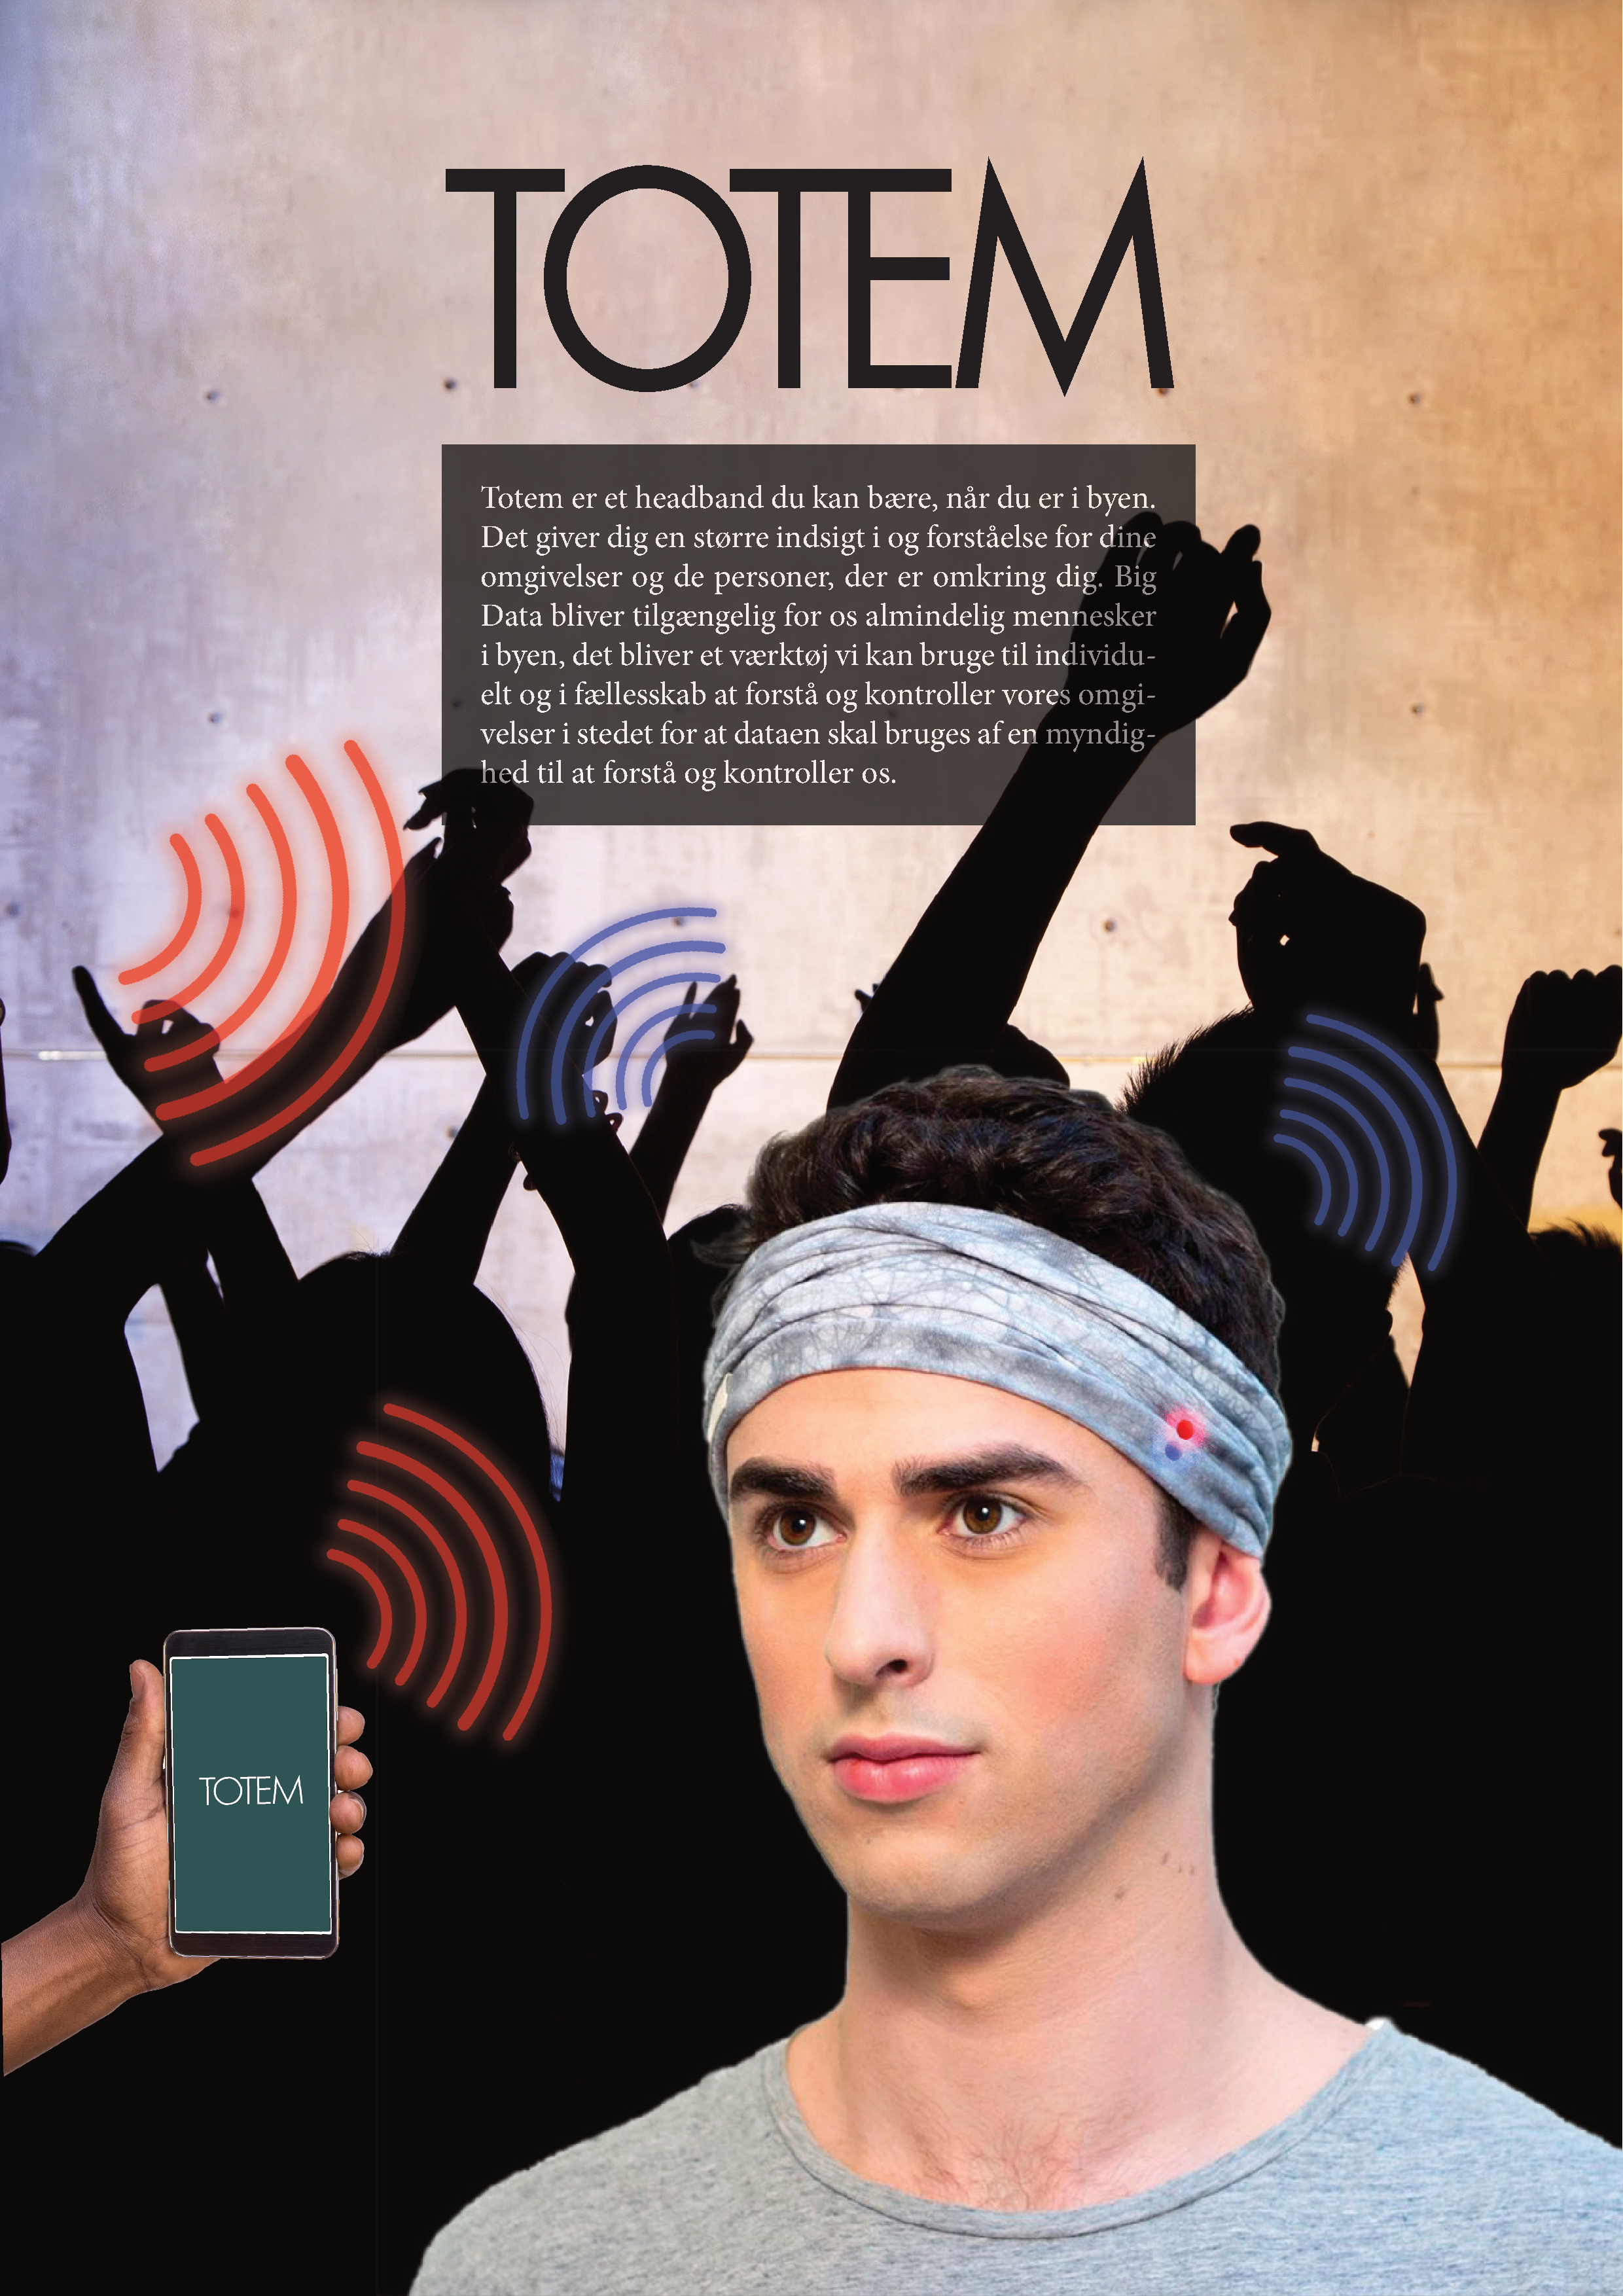
\includegraphics[width = \textwidth]{Pictures/totemplakat.pdf}
    \caption{Plakat brugt til præsentation af TOTEM}
    \label{fig:totemPlakat}
\end{figure}

Denne løsning blev kort og uformelt evalueret med en potentiel bruger. På baggrund af denne og en intern evaluering besluttede vi os, for at bevæge os væk fra konceptet. TOTEM v2 rummede mange af aspekterne fra [b]-listen, men blev ikke acceptere som et reelt produkt, hvorden den ikke formåede at frembringe en kritisk refleksion ved brugeren.

TOTEM tydeliggjorde dog at tryghed kan skabes af flere veje og at der findes forskellige typer for tryghed og man er nødt til at være opmærksom på, hvilken tryghed man sigter imod. Den tryghed TOTEM skaber er meget anderledes end den tryghed predictiv policing skaber. Ved predictive policing kontroller fællesskabet de enkelte individer og sørger for at alle opfører sig efter fællesskabets interesser. Ved TOTEM må hvert individ afgive noget af sig selv til fællesskabet, udvise en tillid til fællesksabet. Med udgangspunkt i dette lavede vi et diagram over typer af trygheder, der kan ses i figur~[FIGUR].


\subsection*{Fictional Inquiry}
På bagrund af dette måtte vi bevæge os længere mod [a]-listens samfundsmodel. Vi ville skabe et scenarie, hvor vi tvang individerne til aktivt at forholde sig til overvågning og big-data i samfund, hvor myndighederne stod for alt tryghed.

Vi afholdte endnu end workshop. Denne gang udførte vi et Fictional Inquiry, som præsenteret af \cite[]{Iversen:2008:PAI:1795234.1795254}. Med inspiration fra [a]-listen opbyggede vi et narrativ som workshoppens fire deltagere sammen med os, skulle leve sig ind i. Deltagerne var hver især var blevet udpeget af PET på baggrund af sammenholdt data om dem. For at virkeliggøre mistanken opbyggede vi rapporterne til hver af deltagerne, som bestod af en blanding af fiktiv og virkelig data om dem. Deltagerne havde intet ulovligt gjort, men narrativet gav PET mulighed at tilbageholde og dømme mistænkte, kun på baggrund af Big Data. Deltagerne havde modtaget et anonymt brev fra en hackergruppe, der havde tilgået deres rapporter før PET kunne pågribe deltagerne. Alle deltagerne blev i brevet bedt om at mødes (til vores workshop) og i fællesskab finde en løsning på deres situation, se billeder i figur~\ref{fig:fictional}.


\begin{figure}

\begin{subfigure}{.5\textwidth}
  \centering
  \includegraphics[width=.8\linewidth]{Pictures/FI1}
    \caption{1}
  \label{fig:sfig1}
\end{subfigure}%
\begin{subfigure}{.5\textwidth}
  \centering
  \includegraphics[width=.8\linewidth]{Pictures/FI2}
    \caption{2}
  \label{fig:sfig1}
\end{subfigure}
\begin{subfigure}{.5\textwidth}
  \centering
  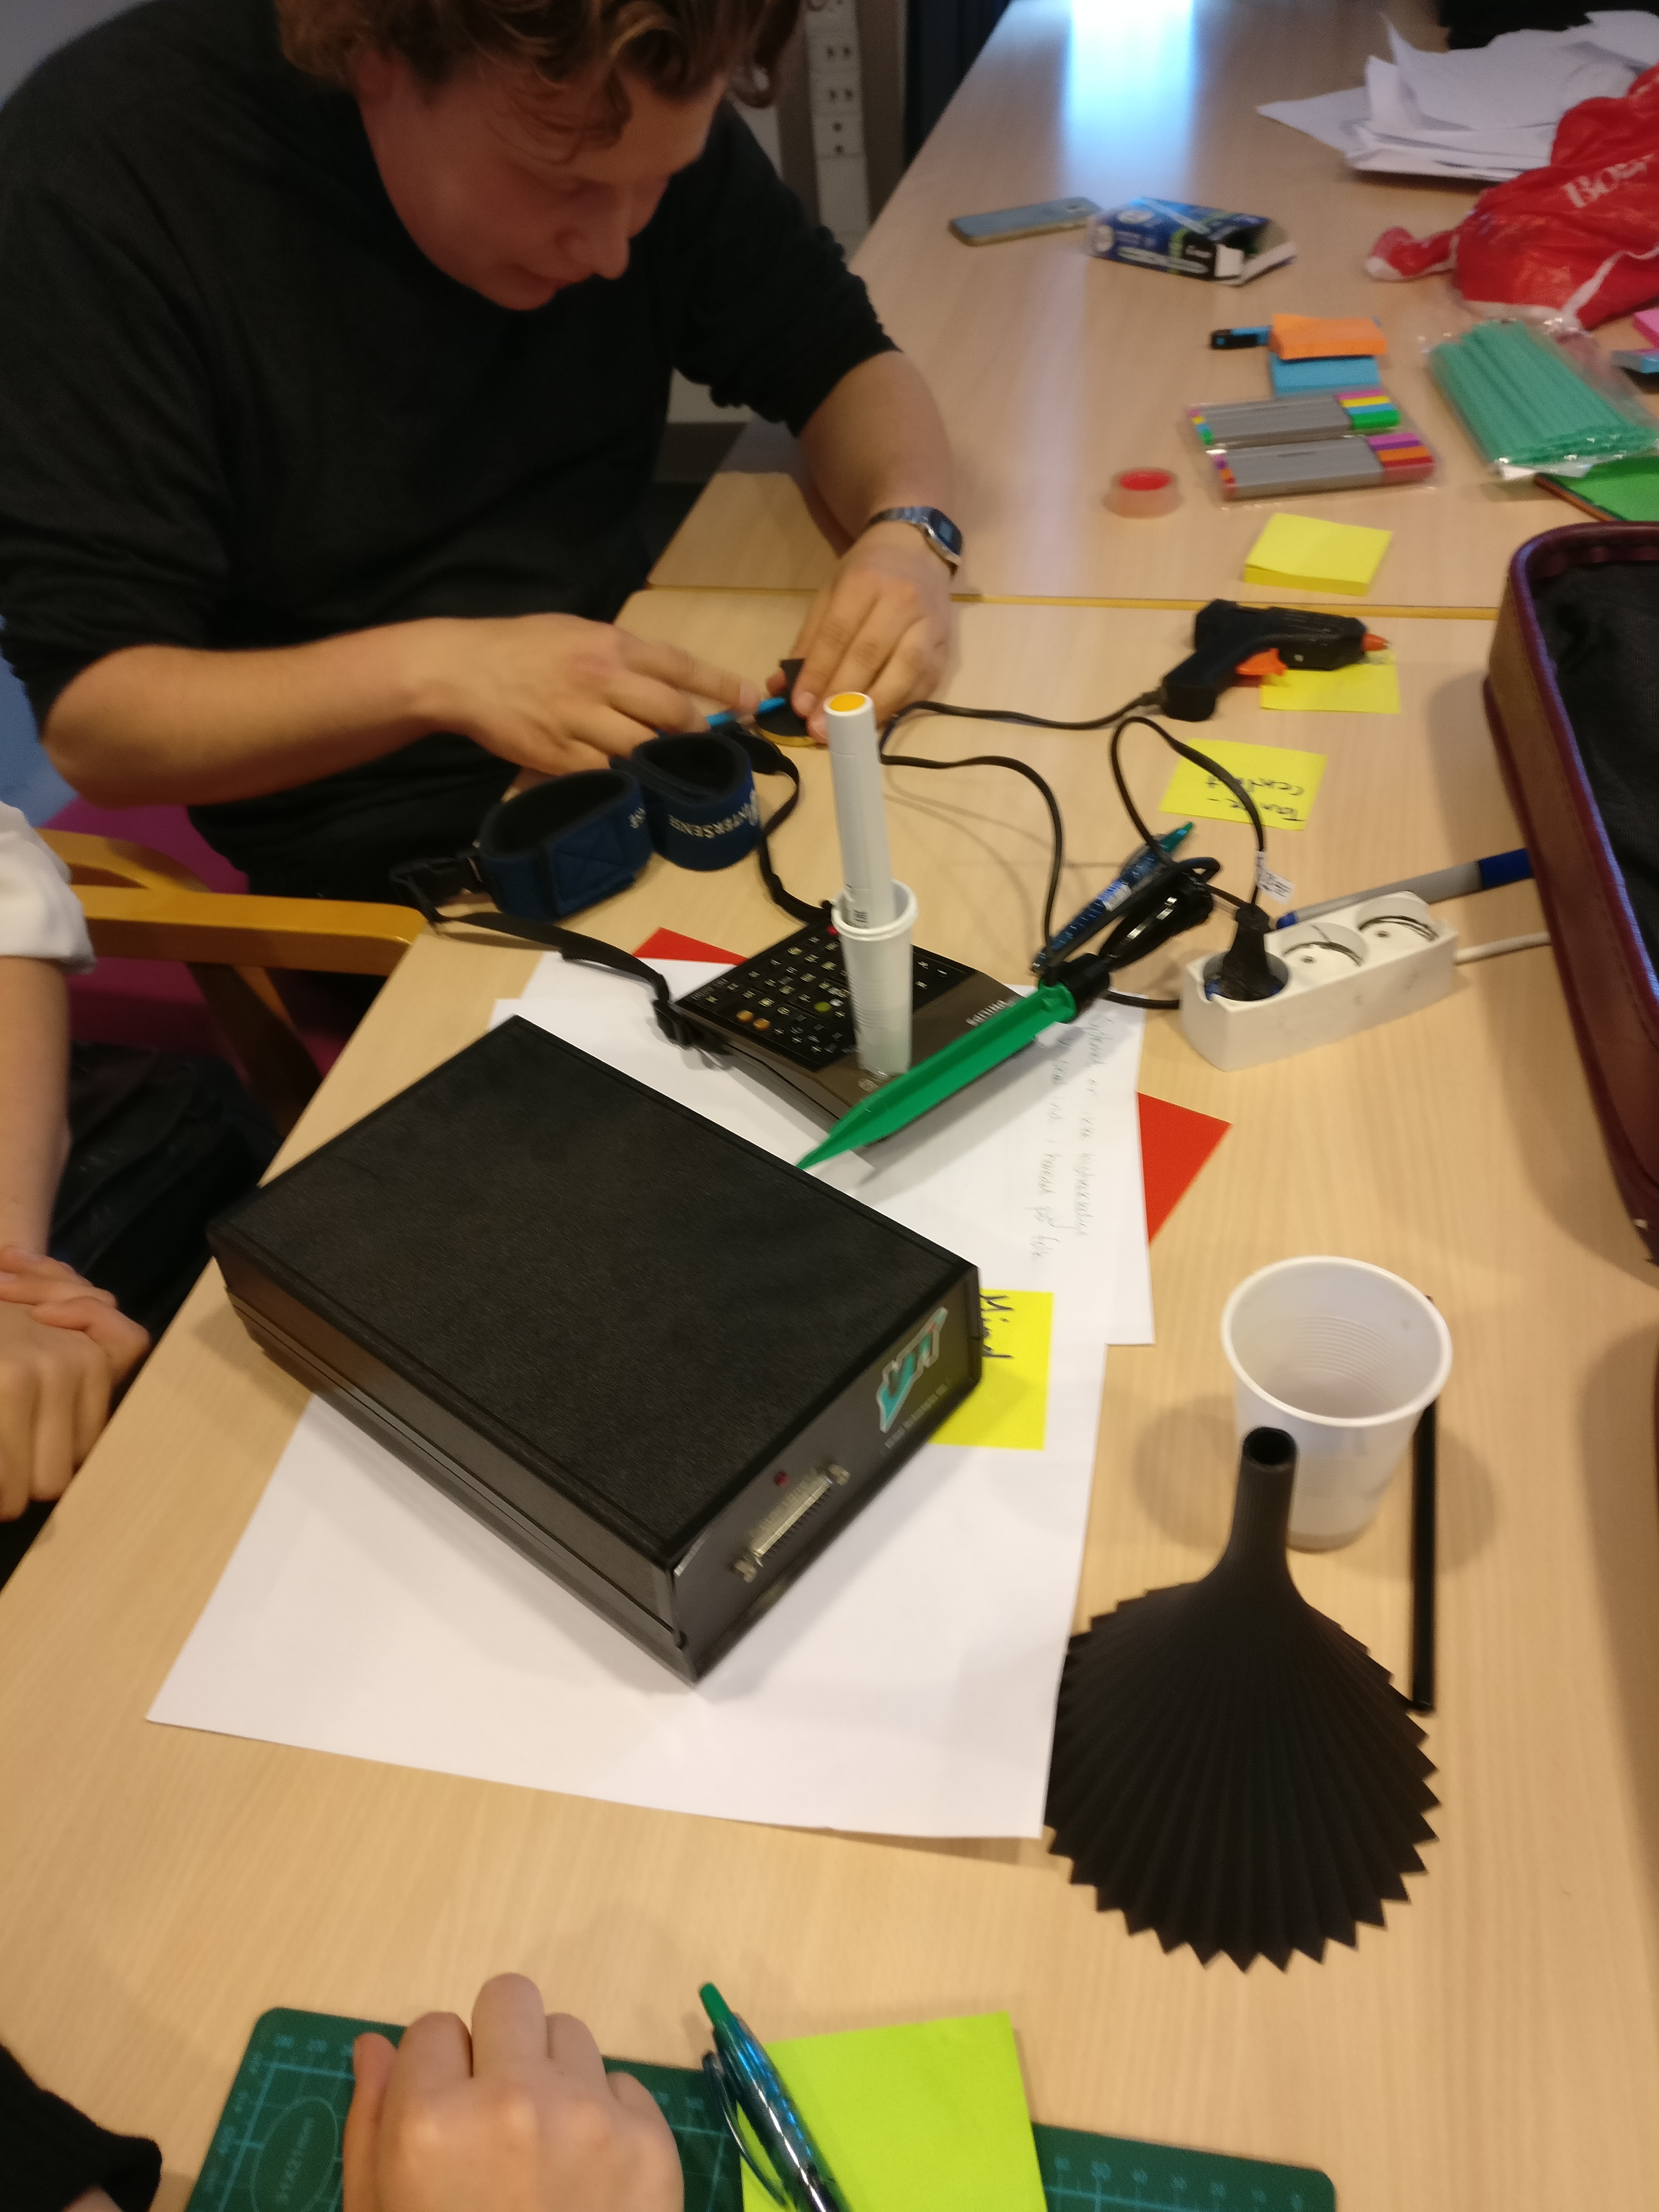
\includegraphics[width=.8\linewidth]{Pictures/FI3}
    \caption{3}
  \label{fig:sfig2}
\end{subfigure}
\begin{subfigure}{.5\textwidth}
  \centering
  \includegraphics[width=.8\linewidth]{Pictures/FI4}
  \caption{4}
  \label{fig:sfig1}
\end{subfigure}%
\caption{Fictional Inquiry workshop, hvor deltagerne er blevet mistænkt på baggrund af Big Data}
\label{fig:fictional}
\end{figure}

Hvordan de ville løse opgaven var frit for. Vi havde fyldt en "spionkuffert" op med genstande, der alle i narrativet kunne bruges til at skabe, slette eller manipulere data. Først gennemgik vi i fællesskab genstandende. Dernæst blev deltagerne delt ind i to grupper og sat i gang. Vi deltog selv i arbejdet i de to grupper på lige fod med de øvrige deltager og sørgede for ikke at dominere processen, men i stedet agere fascilitatorer.

Grupperne udarbejdede en fire prototyper baseret på forskellige ideer om, hvordan PET kunne omgås. Der var især to aspekter, som gik igen i de forskellige prototyper. Først og fremmest var kontrol af data et emne. Alle fire prototyper indebar en skærpet kontrol af den data, der blev opsamlet om en. Dette var dog manifesteret for forskellig vis. I en prototype kunne man åbne en forbindelse til "skyen" og fysisk enten slette eller manipulere sin data ved hjælp af en speciel tang. 

Et andet central emne i workshoppen var \textit{bedre} data. I en prototype kunne man i en personlig databank optage og gemme sine tanker og minder. På denne måde kunne man lagre data som PET og andre overvågere ellers aldrig ville kunne få adgang til. I en anden prototype optog man kontinuerligt data af forskellig art og gemte det på et kassette bånd. Med denne personlige dataopsamler kunne man altså optage data uanset, hvor man var, eller hvad man lavede. Tanken bag begge disse prototyper lavet af to forskellige grupper var, at hvis man kunne optage data, der var \textit{bedre}, altså mere privat eller sværere at få fat på, kunne man konkurrere med det system, der overvågede en.

\subsection*{Den anden iteration}
Narrativet i det udførte Fictional Inquiry viste sig en effektiv måde at få deltagerne til at forholde sig kritisk til brugen af Big Data. Selvom prototyperne, der kom frem under workshoppen er designet ind i en fremskrevet verden, så vi alligevel elementer, der kunne tilbagebringes til en nutidig kontekst uden at miste deres evne til at skabe refleksion. Derfor kombineredes de to centrale elementer fra workshoppen, nemlig ejerskabet og kontrollen over ens egen data samt evnen til at optage og gemme kvalificeret data om en selv, med elementer fra TOTEM konceptet. Fra TOTEM fandt vi inspiration i det stærke fællesskab, produktet skaber. Det enkelte individ står stærkere i kraft af, at fællesskabet og datamængden vokser. I figur~\ref{fig:abakse} vises den serielle proces fra den første workshop frem til dataman.

Derpå designede vi Dataman.

\begin{figure}
    \centering
    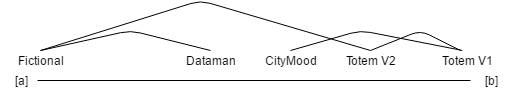
\includegraphics[width = \textwidth]{Pictures/abakse.png}
    \caption{Den serielle proces fra den første workshop frem til dataman}
    \label{fig:abakse}
\end{figure}

%Lave a-b spektre med de forskellige produkter

\begin{comment}



\end{comment}

\section{Diskussion}

\subsection{konceptet}
Sikkerheden i Dataman skulle adresseres stærkt. Der skulle være en stærk End-to-end kryptering mellem enheden og brugerfladen. Teknologien er i dag stærk og udbredt nok til at det ville kunne lykkedes, så dataen var stærkt beskyttet. Man kunne også have valgt at lave en ren trådet forbindelse mellem enheden og ens brugerflade, som måske ville have givet et stærkere æstetisk indtryk, og fornemmelse af at man virkelig har styr på sine data. På den anden side, skulle produktet placeres og forestilles i vores moderne verden, ville det være stærkest med sin trådløse forbindelse mellem alle vores andre trådløse enheder. en trådet forbindelse ville heller ikke forhindre rent fysisk tyveri af sine data, hvor omvendt kan en trådløs forbindelse gøre dette umuligt. 

Håndtrykket for at udveksle data giver også tryghed og en sikkerhed, i og med man fysisk skal have enhederne meget tætte på hinanden for at udveksle denne data. 

I og med 


\begin{comment}
TING AT DISKUTER
    Bruge den teknologi vi har i dag (trådløs)
    
    Hvordan vil dataman ændre vore hverdagoplevelser. Hvordan kandet bruges på nye måder
    HVor er dataman ikke æstetisk (i sin intraktion)
\end{comment}



\setcitestyle{authoryear,open={[},close={]}}

\bibliography{mybib.bib}{}
\bibliographystyle{plainnat}
\end{document}
